%�\pagestyle{fancy}

%\doublespacing

\newcommand{\SHELL}{GridShell}
\newcommand{\AUTHOR}{%
Xi He\\
Rochester Institute of Technology\\
%Bldg 74, Lomb Memorial Drive\\Rochester, NY 14623-5608 \\
Department of Computer Science\\
xi.he@mail.rit.edu%
}
\newcommand{\TITLE}{~\\~\\~\\Improved Parallel Java Cluster Middleware\\~\\~}
\title{\TITLE}
\author{\AUTHOR\\~}
\date{}
\maketitle
%~\\
%~\\
%~\\
%~\\
%~\\
%~\\
%~\\

\vspace{3in}

\begin{minipage}[t]{0.5\textwidth}
~\\
\end{minipage}
\begin{minipage}[t]{0.5\textwidth}
\large{Committee:}\\
~\\
Chair: Prof. Alan Kaminsky\\
Reader: Prof. Hans-Peter Bischof\\
Observer: Prof. Minseok Kwon 
\end{minipage}


\clearpage
%%%%%%%%%%%%%%%%%%%%%%%%%%%%%%%%%%%%%%%%%%%%%%%%%%%%%%%%%%%%%%%%%%%%%%
\section*{Abstract}
%%%%%%%%%%%%%%%%%%%%%%%%%%%%%%%%%%%%%%%%%%%%%%%%%%%%%%%%%%%%%%%%%%%%%%
As CPU clock speed increase has been limited by the cooling techniques and multicore architecture has been widely adopted, Parallel Computing is attracting more and more attention. Parallel Java (PJ) is an API and middleware for parallel programming in 100\% Java developed by Professor Alan Kaminsky. It is running well on cluster parallel computers at Computer Science Department, Rochester Institute of Technology. However, the job launching scheme in PJ is not as efficient as we expect, and it takes a while for PJ to actually start running the submitted jobs. Besides, currently the only way for PJ users to submit their jobs is to log in to the cluster parallel computers and type a few Unix commands via command lines, which has a steep learning curve for people with little computer knowledge.

This project aims to improve the job launching scheme in PJ and make it faster to launch the submitted jobs. Also, the project is targeted at providing PJ users an enhanced Web interface with more functionality.

To achieve our goal, we replace SSH protocol with Message Authentication Codes (MAC) based protocol in the new job launching scheme, redesign the protocol for communication between processes, and implement and evaluate the new job  launching scheme. We also improve the existing Web interface and add to it more functionality such as security, user authentication, session management and job submission. 
\clearpage

\tableofcontents

\clearpage

%\listoffigures

%\listoftables

%\clearpage

%\begin{abstract}
%Your abstract goes here
%\end{abstract}

%%%%%%%%%%%%%%%%%%%%%%%%%%%%%%%%%%%%%%%%%%%%%%%%%%%%%%%%%%%%%%%%%%%%%%
%\section*{Preface}
%%%%%%%%%%%%%%%%%%%%%%%%%%%%%%%%%%%%%%%%%%%%%%%%%%%%%%%%%%%%%%%%%%%%%%

%Put your preface here. 

%%%%%%%%%%%%%%%%%%%%%%%%%%%%%%%%%%%%%%%%%%%%%%%%%%%%%%%%%%%%%%%%%%%%%%
\section{Introduction}
%%%%%%%%%%%%%%%%%%%%%%%%%%%%%%%%%%%%%%%%%%%%%%%%%%%%%%%%%%%%%%%%%%%%%%

As CPU clock speed increase has been limited by the cooling techniques and multicore architecture has been widely adopted, Parallel Computing is attracting more and more attention \cite{sutter2005free}. While the parallel programs are in general written in C, as Java has become one of the most popular languages in the IT industry with its ``write once, run anywhere'' feature and powerful support from open source organizations and big IT vendors, a Java base parallel computing framework is regarded as necessary. 

Parallel Java (PJ) is an API and middleware for parallel programming in 100\% Java developed by Professor Alan Kaminsky \cite{kaminsky2007parallel}. 
Figure \ref{F:architecture} shows the architecture of PJ running on cluster parallel computers with one frontend node and multiple backend nodes connected by a high-speed network.  A Job Scheduler Daemon and multiple Job Frontend Processes run on the frontend nodes. The Job Scheduler Daemon keeps track of each backend node's status and maintains a queue of PJ jobs; The Job Frontend Process connects to the Job Scheduler Daemon, and spawns a Job Backend Process on the backend node. Then the Job Backend Process communicates with Job Frontend Process, obtaining the program�s class files and command line arguments, and calling the static main() method of the main program class. The Job Frontend Process relays the job�s standard input, standard output, and standard error streams between the Job Backend Process and the user�s terminal.  PJ also provides a simple Web interface displaying the status of the cluster parallel computers.

\FIGURE{!htb}
  {images/architecture.pdf}
  {1.0}
  {PJ's Architecture \cite{kaminsky2007parallel}}
  {F:architecture}
  
Currently the Job Frontend Process spawns Job Backend Processes using SSH protocol. Due to the complexity of SSH protocol, the efficiency for this job launching scheme is not as good as we expect. Besides, PJ's Web interface can be improved to allow more user operations. As a result, the goal of our master project is two-fold. One is to design and implement a more efficient job launching scheme. The other is to enable PJ users to perform more tasks via PJ�s web interface, such as job submission. 
 
The remainder of this paper is organized as follows: first we introduce MPI and some of  its important implementation in Section \ref{S:relatedwork}, and describe SSH protocol and our motivation for this project in Section \ref{S:ssh} and \ref{S:motivation}. Then we discuss the design for both the job launching scheme and the Web interface, and implementation issues in Section \ref{S:design} and \ref{S:implementation}. We also present the project deploy instruction, user manual and test result in Section \ref{S:deploy}, \ref{S:usermanual} and \ref{S:test}. Lastly, we propose our future work and conclude the paper in Section \ref{S:futurework} and \ref{S:conclusion}.


%%%%%%%%%%%%%%%%%%%%%%%%%%%%%%%%%%%%%%%%%%%%%%%%%%%%%%%%%%%%%%%%%%%%%%
\section{Related Work \label {S:relatedwork}}
%%%%%%%%%%%%%%%%%%%%%%%%%%%%%%%%%%%%%%%%%%%%%%%%%%%%%%%%%%%%%%%%%%%%%%
 
Message Passing Interface (MPI) \cite{mpi2} is a standard application program interface (API) for writing parallel programs. These MPI programs can run on cluster parallel computers with one process on each node and messages traversing the network between nodes. MPI's feature includes message passing operations, process topologies, multithreading support, one-sided communication and parallel I/O. Typically, a MPI program is a regular C or Fortran program plus calls to the MPI routines to send and receive messages. MPICH2 \cite{mpi}, OpenMPI \cite{openmpi} and Sun MPI \cite{sunmpi} are three important implementations.

\FIGURE{!htb}
  {images/mpijob}
  {0.8}
  {MPI job launching scheme}
  {F:mpijob}
  
Figure \ref{F:mpijob} illustrates MPI's job launching scheme. When a MPI program is submitted to the frontend node, a parent process is spawned and this process calls {\em MPI\_Init} routine for initialization and {\em MPI\_Com\_spawn} routine to spawn child processes on the backend nodes. Once the children processes are created, they call {\em MPI\_Init} routine to initialize MPI communicators for the parent process and the other child processes. Then the MPI program starts launching and messages are passed between the parent process and children processes. When the children processes finish running the program, they return the results to the parent process and the MPI program terminates.
 
PJ is actually a flavor of MPI implementations. Rather than using C or Fortran, PJ is developed purely in Java. Other MPI Java implementations include mpiJava \cite{mpijava} and MPJ \cite{baker-mpj}.  mpiJava and MPJ both stick to MPI standard. However, mpiJava is implemented as a thin Java native interface while MPJ is a 100\% Java implementation. 

In \cite{kaminsky2009building}, Professor Kaminsky tried to compare MPI and PJ by running a C program of Floyd's Algorithm on a Sun MPI Library and a Java program of Flod's Algorithm on PJ. The result shows the Java program's running times are about 50 percent higher than the C program's running times.  In Section \ref{S:test}, we measure the time for both PJ and MPI to start launching jobs and compare their efficiency. 


%%%%%%%%%%%%%%%%%%%%%%%%%%%%%%%%%%%%%%%%%%%%%%%%%%%%%%%%%%%%%%%%%%%%%%
\section{SSH \label {S:ssh}}
%%%%%%%%%%%%%%%%%%%%%%%%%%%%%%%%%%%%%%%%%%%%%%%%%%%%%%%%%%%%%%%%%%%%%%
Secure Shell or SSH is a network protocol that allows data to be exchanged using a secure channel between two networked devices. The initial version, SSH1, focused on providing a secure remote logon facility to replace Telnet and other remote logon schemes that provided no security. The new version, SSH2, provides a standardized definition of SSH and improves on SSH1 in numerous ways. 

\FIGURE{!htb}
  {images/ssh_architecture}
  {0.8}
  {SSH Protocol Architecture}
  {F:ssh_architecture}

Typically running on top of TCP protocol, SSH \cite{ssh} is organized into three layers of protocol: Transport Layer Protocol, User Authentication Layer Protocol and Connection Layer Protocol, as shown in Figure \ref{F:ssh_architecture}.  Transport Layer Protocol is responsible for server authentication, confidentiality and integrity. On top of Transport Layer Protocol, User Authentication Layer Protocol authenticate the user to the server and then Connection Layer Protocol multiplexes logical communications channels over a single underlying SSH connection.

\subsection{Transport Layer Protocol}

\FIGURE{!htb}
  {images/ssh_transport}
  {0.8}
  {The typical message sequences in SSH Transport Protocol}
  {F:ssh_transport}

Figure \ref{F:ssh_transport} illustrates the typical message sequences in the SSH Transport Layer \cite{ssh-userauth}. First, the client establishes a TCP connection to the server. When the connection is established, the client and the server can start to exchange data.  The first step of data exchange, the identification string exchange, begins with the client sending its identification string composed of the version number of SSH protocol and SSH implementation. The server then responds with its identification string. 

The next step of data exchange is algorithm negotiation. Both the client and the server send the other side SSH\_MSG\_KEXINIT message containing lists of supported algorithms in the order of preference to the sender. The types of algorithms that need to negotiation include key exchange, encryption, MAC algorithm and compression algorithm. Each type of algorithms has one list of available algorithm to choose from. For each category of algorithm, the first algorithm on the client's list that is supported by the server will be chosen. 

The step of key exchange comes after algorithm negotiation. At present two versions of Diffie\_Hellman key exchange algorithm are specified. Three sub-steps are involved in key exchange and they are explained as follows. Here, $p$ denotes a large safe prime; $g$ denotes a generator for a subgroup of of $GF(p)$; $q$ is the order of subgroup. 

\begin{itemize}
\item The client generates a random number $x (1< x< q)$ and computes $e=g^x$ mod $p$. Then send the server a SSH\_MSG\_NEWKEYS message containing $e$.
\item The server receives $e$, and it also generates a random number $y (0<y<q)$ and computes $f=g^y$ mod $p$. Then the server can compute the exchanged key $K=e^y$ mod $p$. The server hashes the client's SSH\_MSG\_KEXINIT message, the server's SSH\_MSG\_KEXINIT message, the client's identification, the server's identification, the server's public host key, $e$, $f$ and $K$ into $H$ and signature $s$ on $H$ using its private host key. The server send back a SSH\_MSG\_NEWKEYS message containing  $f$, $s$ and the server's public host key.
\item The client receives the message from the server and verifies that the public host key is the authenticate host key for the server it want to connect by means of searching the key in the local host key database. Then the client can computer $K=f^x$ mod $p$. The client also calculate $H$, the hash value of the client's SSH\_MSG\_KEXINIT message, the server's SSH\_MSG\_KEXINIT message, the client's identification, the server's identification, the server's public host key, $e$, $f$ and $K$.  After verifying with $s$, the client can trust the server.
\end{itemize} 

As a result of above steps, the client and the server now share a master key $K$. In addition, the server is authenticated by the client. As a final step in the Transport Layer Protocol, the client sends the SSH\_MSG\_SERVICE\_REQUEST to the server to request the user authentication service. And the server response with  SSH\_MSG\_SERVICE\_ACCEPT message. Subsequent to these messages, all data exchanged are protected by encryption and MAC.

\subsection{User Authentication Layer Protocol}
\FIGURE{!htb}
  {images/ssh_authentication}
  {0.8}
  {The typical message sequences in User Authentication Layer Protocol}
  {F: ssh_authentication}
  
Figure \ref{F: ssh_authentication} illustrates the message sequences in User Authentication Layer Protocol\cite{ssh-transport}. The explanation is as follows: 

\begin{enumerate}
   \item The client sends a SSH\_MSG\_USERAUTH\_REQUEST message containing the username and a ``requested method'' of none.
   \item The server checks the validity of the username. If username is not valid, the server returns SSH\_MSG\_USERAUTH\_FAILURE with ``the partial success value'' of false, and terminates the conversation.
   \item If the username is valid, the server returns SSH\_MSG\_USERAUTH\_FAILURE with ``the partial success value'' of true and a list of one or more authentication methods to be used.
   \item The client selects one of the acceptable authentication methods and informs the server of the authentication method name through a SSH\_MSG\_USERAUTH\_REQUEST message. Then the client and the server will exchange the required method-specific fields by a sequence of SSH\_MSG\_USERAUTH\_INFO\_REQUEST and SSH\_MSG\_USERAUTH\_INFO\_RESPONSE message passing. 
   \item If the authentication on the selected authentication methods fails, the client will try another authentication method. If the client already tries all of the acceptable authentication methods, the authentication fails and the conversation is terminated.
   \item If the authentication succeeds, the server sends a SSH\_MSG\_USERAUTH\_SUCCESS message to the client.
\end{enumerate}
 
\subsection{Connection Layer Protocol}

\FIGURE{!htb}
  {images/ssh_connection}
  {0.8}
  {The typical message sequences in Connection Layer Protocol}
  {F: ssh_connection}
  
The SSH Connection Layer Protocol \cite{ssh-connect} runs on top of the SSH Transport Layer Protocol and assumes that the User Authentication Protocol has been invoked. The Connection Layer Protocol supports a number of logical channels and all types of communication using SSH are supported using separate channels. Here is how Connection Layer Protocol works (Figure \ref{F: ssh_connection}):

\begin{enumerate}
   \item The client sends the server a SSH\_MSG\_CHANNEL\_OPEN message to request the open of a new channel. The message includes the channel type, sender channel number, initial window size and maximum packet size 
   \item If the server is able to open the channel, it return a SSH\_MSG\_CHANNEL\_OPEN\_CONFIRMATION message including the sender channel number, the recipient channel number, and window and packet size values for incoming traffic. 
   \item Once a channel is open, data transfer on both sides is performed using SSH\_MSG\_CHANNEL\_DATA messages.
   \item When the client wishes to close the channel, it sends a SSH\_MSG\_CHANNEL\_CLOSE message to the server and then the channel is close.
\end{enumerate}

%%%%%%%%%%%%%%%%%%%%%%%%%%%%%%%%%%%%%%%%%%%%%%%%%%%%%%%%%%%%%%%%%%%%%%
\section{Motivation \label {S:motivation}}
%%%%%%%%%%%%%%%%%%%%%%%%%%%%%%%%%%%%%%%%%%%%%%%%%%%%%%%%%%%%%%%%%%%%%%
%\begin{figure}[htb]
%    \centerline{
%    \subfigure[SSH Protocol Architecture ]{\label{F:ssh_architecture}{\resizebox{0.5\linewidth}{!}{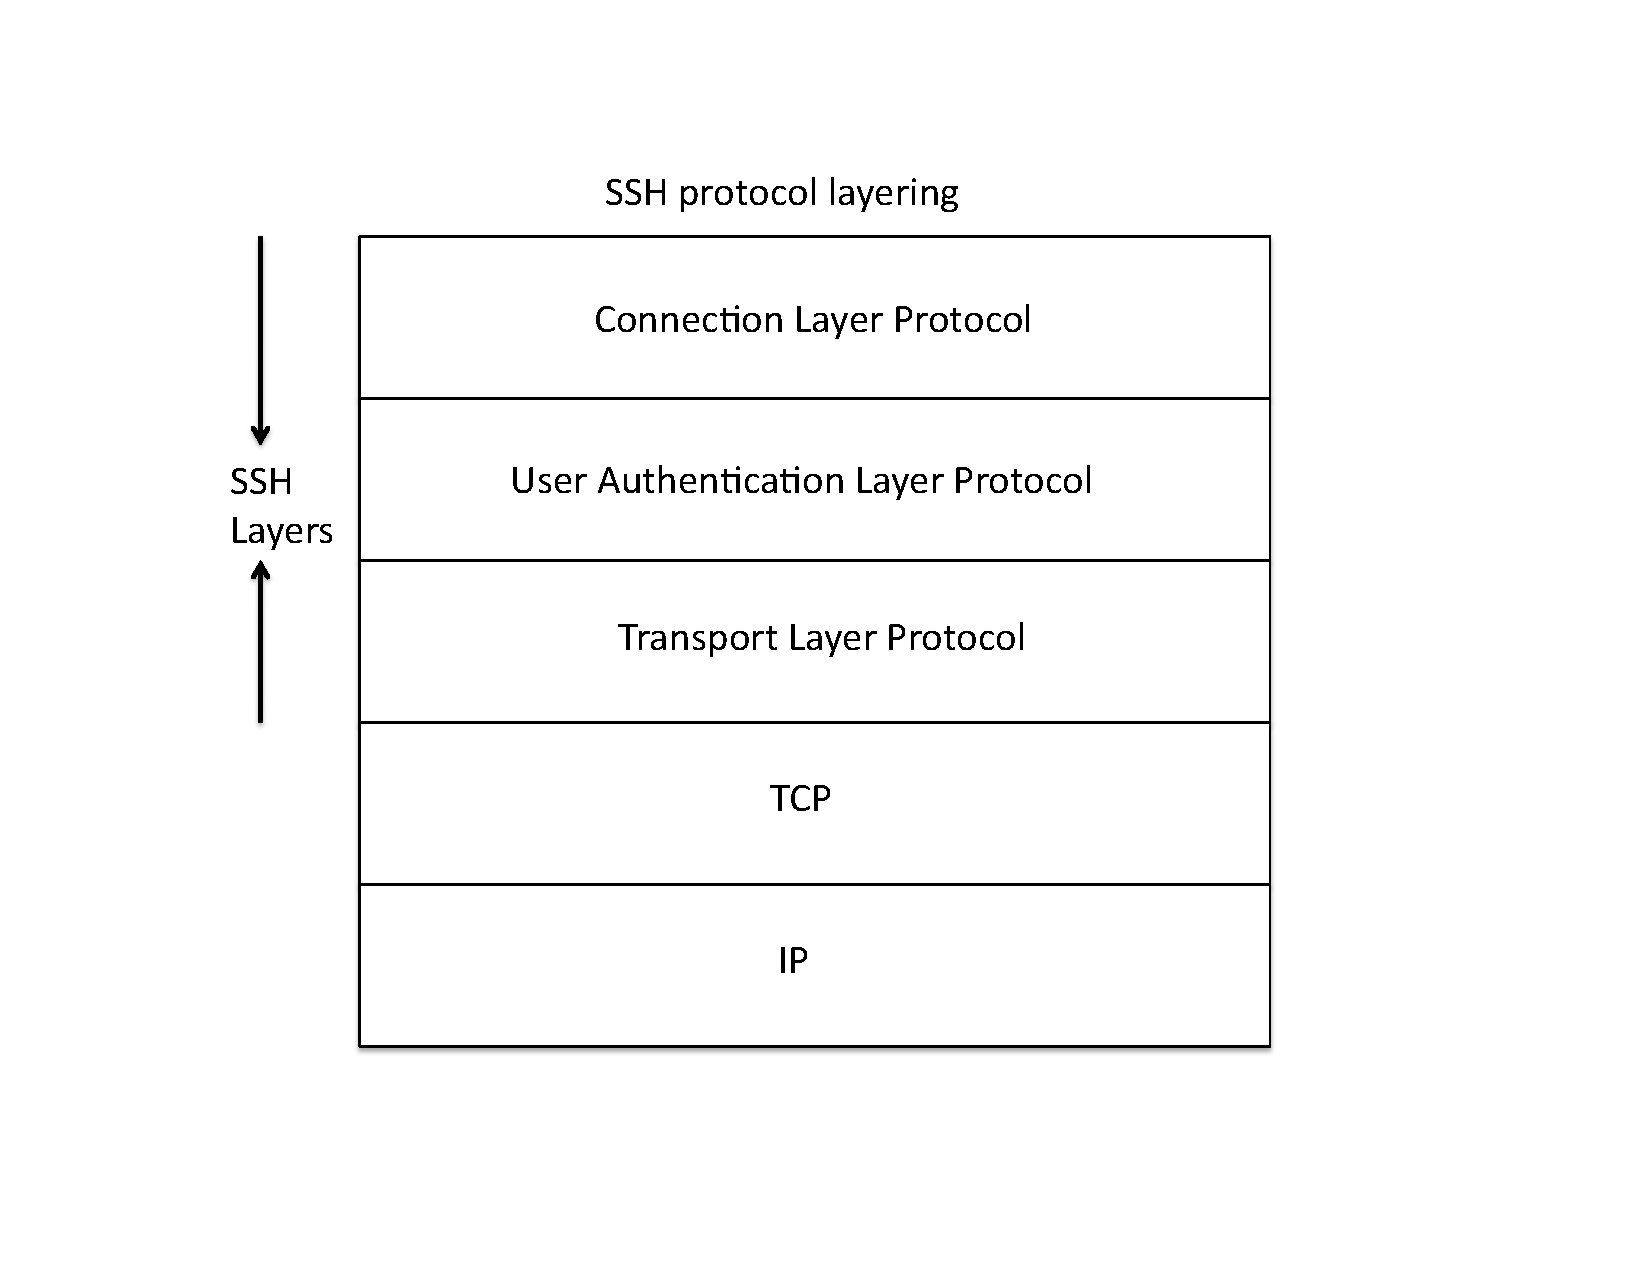
\includegraphics{images/ssh_architecture}}}}
%    %\subfigure[b]{\label{F:dvfs2}{\resizebox{0.3\linewidth}{!}{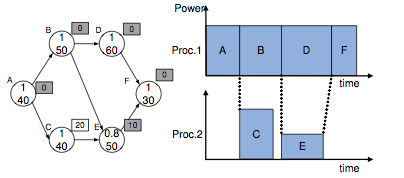
\includegraphics{images/dvfs2}}}}
%    \subfigure[SSH Protocol Flow]{\label{F:ssh_flow}{\resizebox{0.5\linewidth}{!}{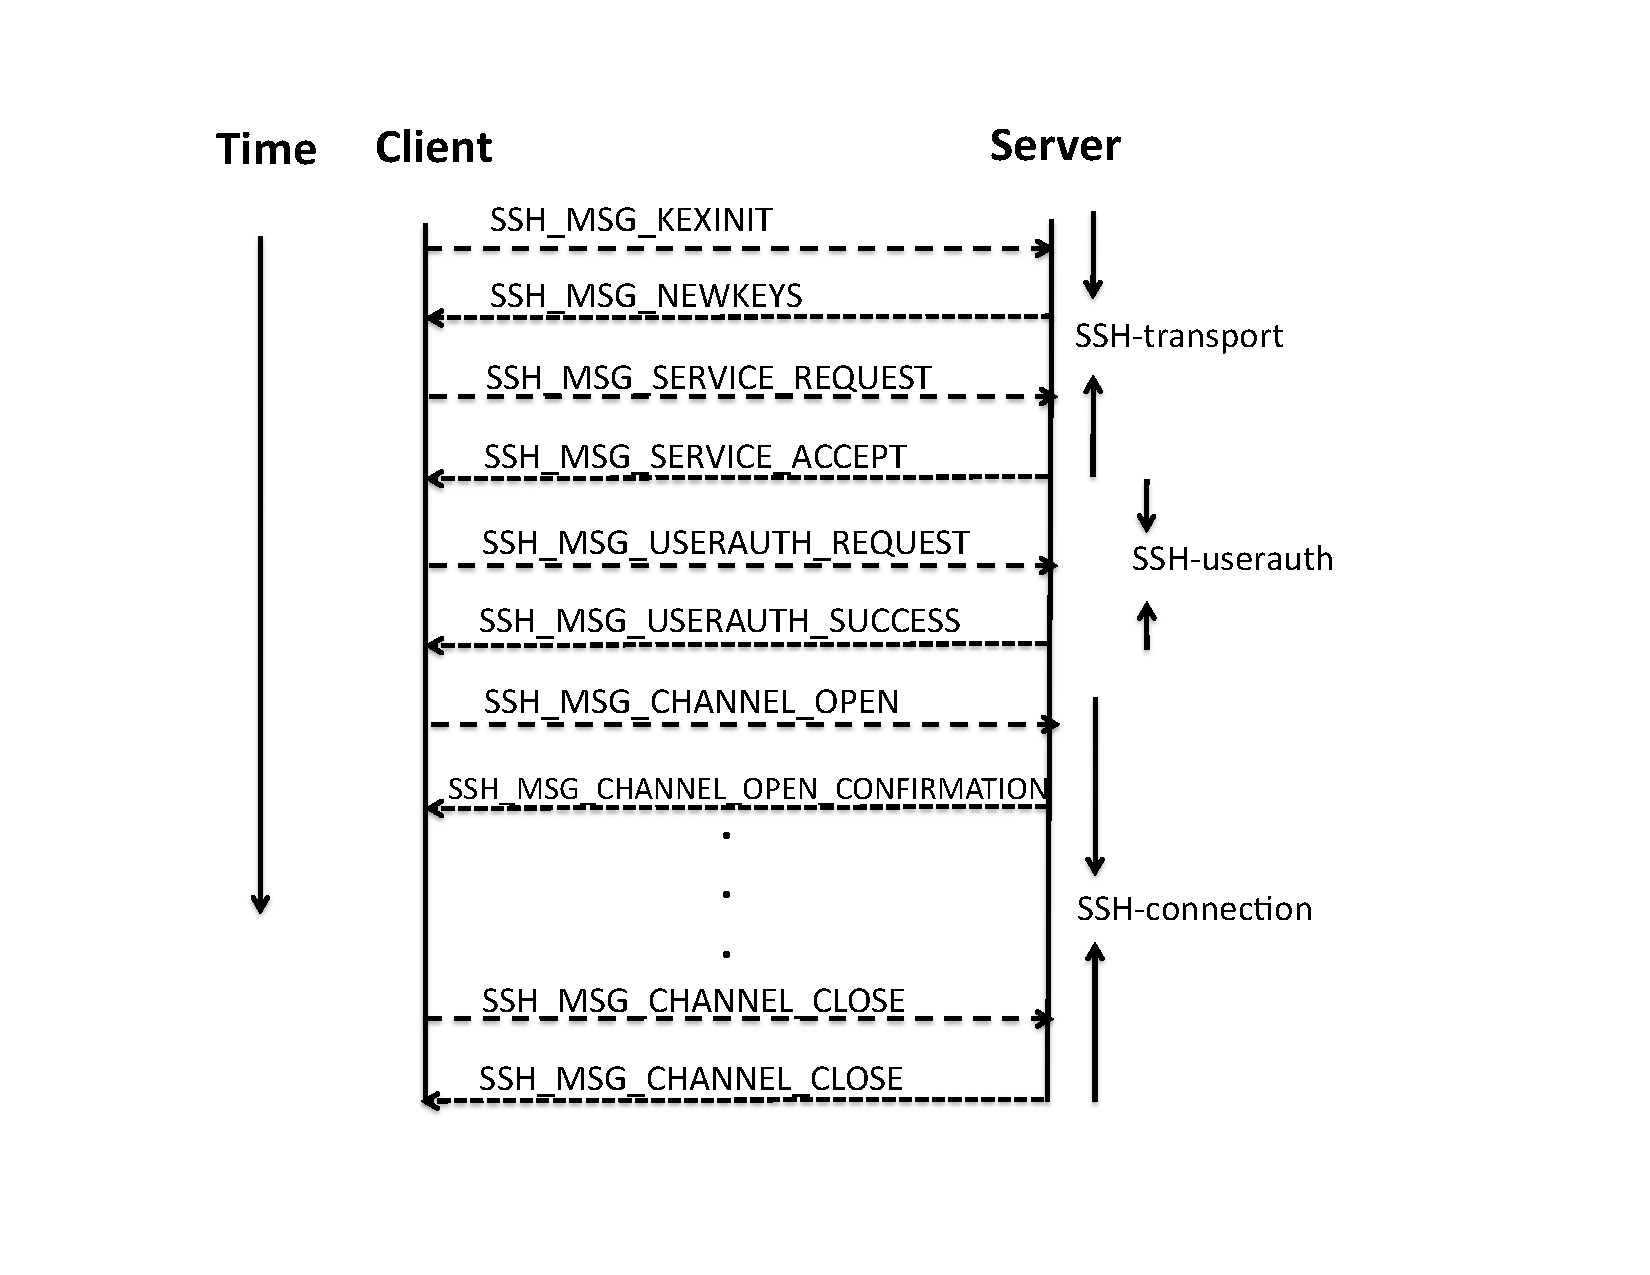
\includegraphics{images/ssh}}}}
%    }
%\caption {SSH Protocol }
%\label {F:ssh}
%\end{figure}

The original job launching scheme relies on SSH protocol to spawn new Job Backend Processes to execute the submitted job. As we discuss in Section \ref{S:ssh}, SSH protocol is a powerful and complicated protocol. It involves encryption, both sides authentication, key exchange, data integrity, data compression and other functionality. However, PJ's job launching scheme only needs part of functionality that SSH provides. For example, PJ does not need to encrypt its messages because  these messages do not contain any confidential information. Also, PJ does not necessarily need algorithm exchange or key exchange. We can predefine algorithm or preconfigure cryptographic key for the communication between computer nodes. These unnecessary functionalities makes PJ's job launching scheme much less efficient. Actually only the both sides authentication and data integrity verification are what PJ's job launching scheme essentially needs.


In addition, Parallel Computing is often applied to other disciplines which need massive computational power, such as physics, biology and astronomy. It might be painful for scientists in these disciplines to work in Unix-like system. A interactive Web interface will be helpful, because people can utility computational power without any prerequisite and submit their jobs just like surfing the Internet.  The original PJ's Web interface only provides limited functionality and there is much room for improvement. 

%%%%%%%%%%%%%%%%%%%%%%%%%%%%%%%%%%%%%%%%%%%%%%%%%%%%%%%%%%%%%%%%%%%%%%
\section{Design \label {S:design}}
%%%%%%%%%%%%%%%%%%%%%%%%%%%%%%%%%%%%%%%%%%%%%%%%%%%%%%%%%%%%%%%%%%%%%%
\subsection{Job Launching Scheme}
\subsubsection{Overview}
The basic idea behind the design of the new job launching scheme is that we try to avoid using SSH protocol to spawn the Job Backend Processes. Instead, we use MAC based message to inform backend nodes to run the submitted jobs.

\FIGURE{!htb}
{images/newarchitecture}
{1}
{PJ's New Architecture}
{F:newarchitecture}

Figure \ref{F:newarchitecture} shows PJ's new architecture based on which the job launching scheme is improved. A Job Scheduler Daemon is always running on the frontend node, and listening for connections to a well-known port; When each end user logs in to the frontend node and tries to run his parallel programs, a Job Frontend Process is actually created and this Job Frontend Process then communicates with the Job Scheduler Daemon and requests computing resources to run the submitted job;  If being allocated enough computing resources, the Job Frontend Process begins to communicates with Job Backend Daemons on those assigned backend nodes. The Job Backend Daemons are running on a per user basis. So there might be multiple Job Backend Daemons running on behalf of different users at the same time. The Job Frontend Process might need to use SSH to spawn a Job Backend Daemons if there is no corresponding Job Backend Daemon running. Once the authentication between the Job Frontend Process and the Job Backend Daemon is finished, the Job Backend Daemon will spawn the Job Backend Process.  

Next, we present the details of the protocols between different processes.
\subsubsection{Protocol design}

\paragraph{Protocol for Job Scheduler Daemon and Job Frontend Process}

\FIGURE{!htb}
{images/protocol1}
{0.8}
{Communication between Job Scheduler Daemon and Job Frontend Process}
{F: protocol1}

Figure \ref{F: protocol1} illustrates the communication protocol between Job Scheduler Daemon and Job Frontend Process. As a Job Frontend Process is created, it sends the Job Scheduler Daemon a ``Request job'' message containing the name of the user and the required number of processors. The Job Scheduler Daemon gets the message and checks the resource pool to see if the overall computing resources are sufficient for the job.  If there are not enough computing resources, the Job Scheduler Daemon sends back a ``Cancel job'' message and terminates the conversation. If there exist sufficient computing resources, the Job Scheduler Daemon puts the job into its job queue. The job queue follows the FIFO policy and when it is the job's turn to run, the Job Scheduler Daemon assigns the idle backend nodes to the job. If there is a Job Backend Daemon running as the same user as the job submitter on the backend nodes, the Job Scheduler Daemon will send the Job Frontend Process a ``Assign Backend Daemon'' message. Otherwise, the Job Scheduler Daemon sends a ``Create Backend Daemon'' message to the Job Frontend Process.  Since then, the Job Frontend Process begins to communicate with the Job Backend Daemon and the Job Backend Process until the job is finished. When the job is done, the Job Frontend Process tells the Job Scheduler Daemon ``Job finished''.

The Job Scheduler Daemon renews a lease on the Job Frontend Process, and vice versa, by sending a "renew lease" message every 60 seconds. If some failure is detected during job execution, the Job Scheduler Daemon or the Job Frontend Process can send the other side a ``Cancel job'' message to terminate the conversation. 

\paragraph{Protocol  for Job Frontend Process and Job Backend Daemon}
\FIGURE{!htb}
{images/protocol2}
{0.8}
{Communication between Job Frontend Process and Job Backend Daemon}
{F: protocol2}

Figure \ref{F: protocol2} illustrates the communication protocol between Job Frontend Process and Job Backend Daemon. When the Job Frontend Process receives the ``Assign Backend Daemon'' message from the Job Scheduler Daemon, it will try to communicate with the Job Backend Daemon. Since these two processes run in two different computer nodes and communicate through message passing, We need a two sides authentication mechanism and avoid security issues. For this project, we adopt the challenge-response MAC based authentication\cite{mac}. 

\FIGURE{!htb}
{images/mac}
{0.6}
{Message Authentication Codes}
{F: mac}
A message authentication code (MAC) is a short piece of information used to authenticate a message. We choose HMAC \cite{hmac} algorithm, a hash function based MAC algorithm, as the authentication and integrity algorithm. The selected hash function is SHA-256\cite{standard2002federal}. Figure \ref{F: mac} explains how HMAC algorithm works. An authentication key and an arbitrary-length message are inputed to the HMAC-SHA-256 hash function to generate the fixed-length HMAC. Only the same input message and authentication key can generate the same HMAC.  For this reason, the HMAC message can be used for authentication and data integrity. The following steps show how we use HMAC to achieve both sides authentication and data integrity verification.

\begin{itemize}
\item As we will mention in Section \ref{S:usermanual}, before starting to submit jobs to PJ, each user needs to generate his own authentication key and save the key in the {\em key} file under .ssh/hmac/ on his account. The user also needs to configure the privilege of {\em key} file and make it only accessible to the user. 	 
\item When the Job Frontend Process and the Job Backend Daemon start, they read the authentication key from the {\em key} file.  
\item The Job Frontend Process generates a random number A, and sends A to the Job Backend Daemon. 
\item The Job Backend Daemon receives the random number A. It also generates another random number B. Then it computes MAC(A$\mid$B) using the authentication key K and gets a message authentication code MAC1. It sends MAC1 and B to the Job Frontend Process.
\item When the Job Frontend Process receives MAC1 and B, it computes MAC(A$\mid$B) using the authentication key K and gets a message authentication code MAC2. Comparing MAC1 with MAC2 and if MAC1!=MAC2, the Job Frontend Process thus terminates the conversation. Otherwise,  the Job Frontend Process computes MAC(A$\mid$B$\mid$Job info) using the authentication key K and gets a message authentication code MAC3. The job information includes user JVM command line flags, username, job number, the required number of processors, the Job Backend Process's rank, the flag of whether there exists a Job Backend Process's frontend communicator, the hostname and the port number of the Job Frontend Process, and the hostname of the backend node. Then it sends MAC3 and these job information to the Job Backend Daemon.
\item When the Job Backend Daemon receives the job information and MAC3, it computes MAC(A$\mid$B$\mid$Job info) using the authentication key K and gets a message authentication code MAC4. It then compares MAC3 with MAC4. If MAC3!=MAC4, the Job Backend Daemon terminates the conversation. Otherwise the Job Backend Daemon begin to spawn a new Job Backend Process with the provided job information. Here is how  the Job Backend Daemon spawn the new Job Backend Process:

When a Job Backend Daemon is created by Job Frontend Process, the Job Frontend Process specified the full pathname of JVM at the backend node, the class path for PJ library and JVM command line flags. With these information and the job information passed by the Job Frontend Process, the Job Backend Daemon can construct the command string as follows:
\small
\begin{verbatim}
<jvm> -classpath <classpath>  <jvmflags>  edu.rit.pj.cluster.JobBackend \
<args> >/dev/null 2>/dev/null & 
\end{verbatim} 
\normalsize
\textless jvm\textgreater=JVM pathname; \textless jvmflags\textgreater=JVM command line flags, including the user JVM command line flags; \textless classpath\textgreater=Java class path for PJ library; \textless args\textgreater=job information which is passed by Job Frontend Process.

Thus Job Backend Daemon runs this command and spawn a new Job Backend Process with the provided job information. 
\end{itemize}


\paragraph{Protocol  for Job Scheduler Daemon and Job Backend Daemon}
\FIGURE{!htb}
{images/protocol3}
{0.8}
{Communication between Job Scheduler Daemon and Job Backend Daemon}
{F: protocol3}
Figure \ref{F: protocol3} illustrates the communication protocol between Job Scheduler Daemon and Job Backend Daemon.The communication between Job Scheduler Daemon and Job Backend Daemon is to let Job Scheduler Daemon keep track of the status of Job Backend Daemons

\begin{itemize}
\item When a new Job Backend Daemon is created, it sends Job Scheduler Daemon a ``Ready'' message and tells the Job Scheduler Daemon its IP address, port number and the name of user who owns the Job Backend Daemon. 
\item Each of the running Job Backend Daemons sends a ``renew lease'' message to the Job Scheduler Daemon every 60 second and informs the Job Scheduler Daemon that it is still running. 
\item If no Job Frontend Process communicates with the Job Backend Daemon in 600 seconds, the Job Backend Daemon will send Job Scheduler Daemon a ``terminate'' message and tells the Job Scheduler Daemon that it is going to terminate.
\end{itemize}




\paragraph{Protocol for Job Frontend Process and Job Backend Process}
\FIGURE{!htb}
{images/protocol4}
{0.8}
{Communication between Job Frontend Process and Job Backend Process }
{F: protocol4}

Figure \ref{F: protocol4} illustrates the communication protocol between Job Frontend Process and Job Backend Process. The Job Backend Process begins by sending a "backend ready" message to the Job Frontend Process. 
Once all the Job Backend Processes have reported ready, the Job Frontend Process sends a "commence job" message to each Job Backend Process and tell them to start running. The Job Backend Process sends a ``request resource'' message to load the user's program and the Job Frontend Process respond with a ``report resource'' message and transport the bytecodes to the Job Backend Process. Since then, the Job Backend Process starts running the user' program. When the job is done, the Job Backend Process sends Job Frontend Process a ``Backend finished'' message. Once all the Job Backend Processes have reported that they have finished their jobs, the Job Frontend Process sends each Job Backend Process a ``Job finished'' message. 

The Job Frontend Process renews a lease on the Job Backend Process, and vice versa, by sending a ``renew lease" message every 60 seconds. If some failure is detected during job execution, the Job Frontend Process or the Job Backend Process can send the other side a ``Cancel job'' message to terminate the conversation. 

%\subsubsection{Remote Method Calls in PJ}
%\FIGURE{!htb}
%{images/rmi}
%{0.8}
%{Remote Method Invocation Framework }
%{F: rmi}

%PJ is a distributed system and composed of multiple distributed objects running on cluster parallel computers. These distributed objects communicate with each other using the protocol we discussed above. Here we discuss the remote method calls in PJ. 

%For example, in Figure \ref{F: rmi}, object {\em A} and object {\em B} are in different computer nodes, and object B is going to call the method {\em m1} in object {\em A}. To do this, object {\em B} creates a message object including the method name and the method arguments, and sends this message to object {\em A} via {\em Proxy} object over the {\em Channel} between {\em A} and {\em B}. When object {\em A} receives this message, it extracted the method name and method arguments from the message, and execute this method with provided arguments.

\subsection{Web interface}
 \subsubsection{Authentication Issues} 
\begin{figure}[htb]
    \centerline{
    \subfigure[Fail to spawn user B's process]{\label{F:auth_fail}{\resizebox{0.5\linewidth}{!}{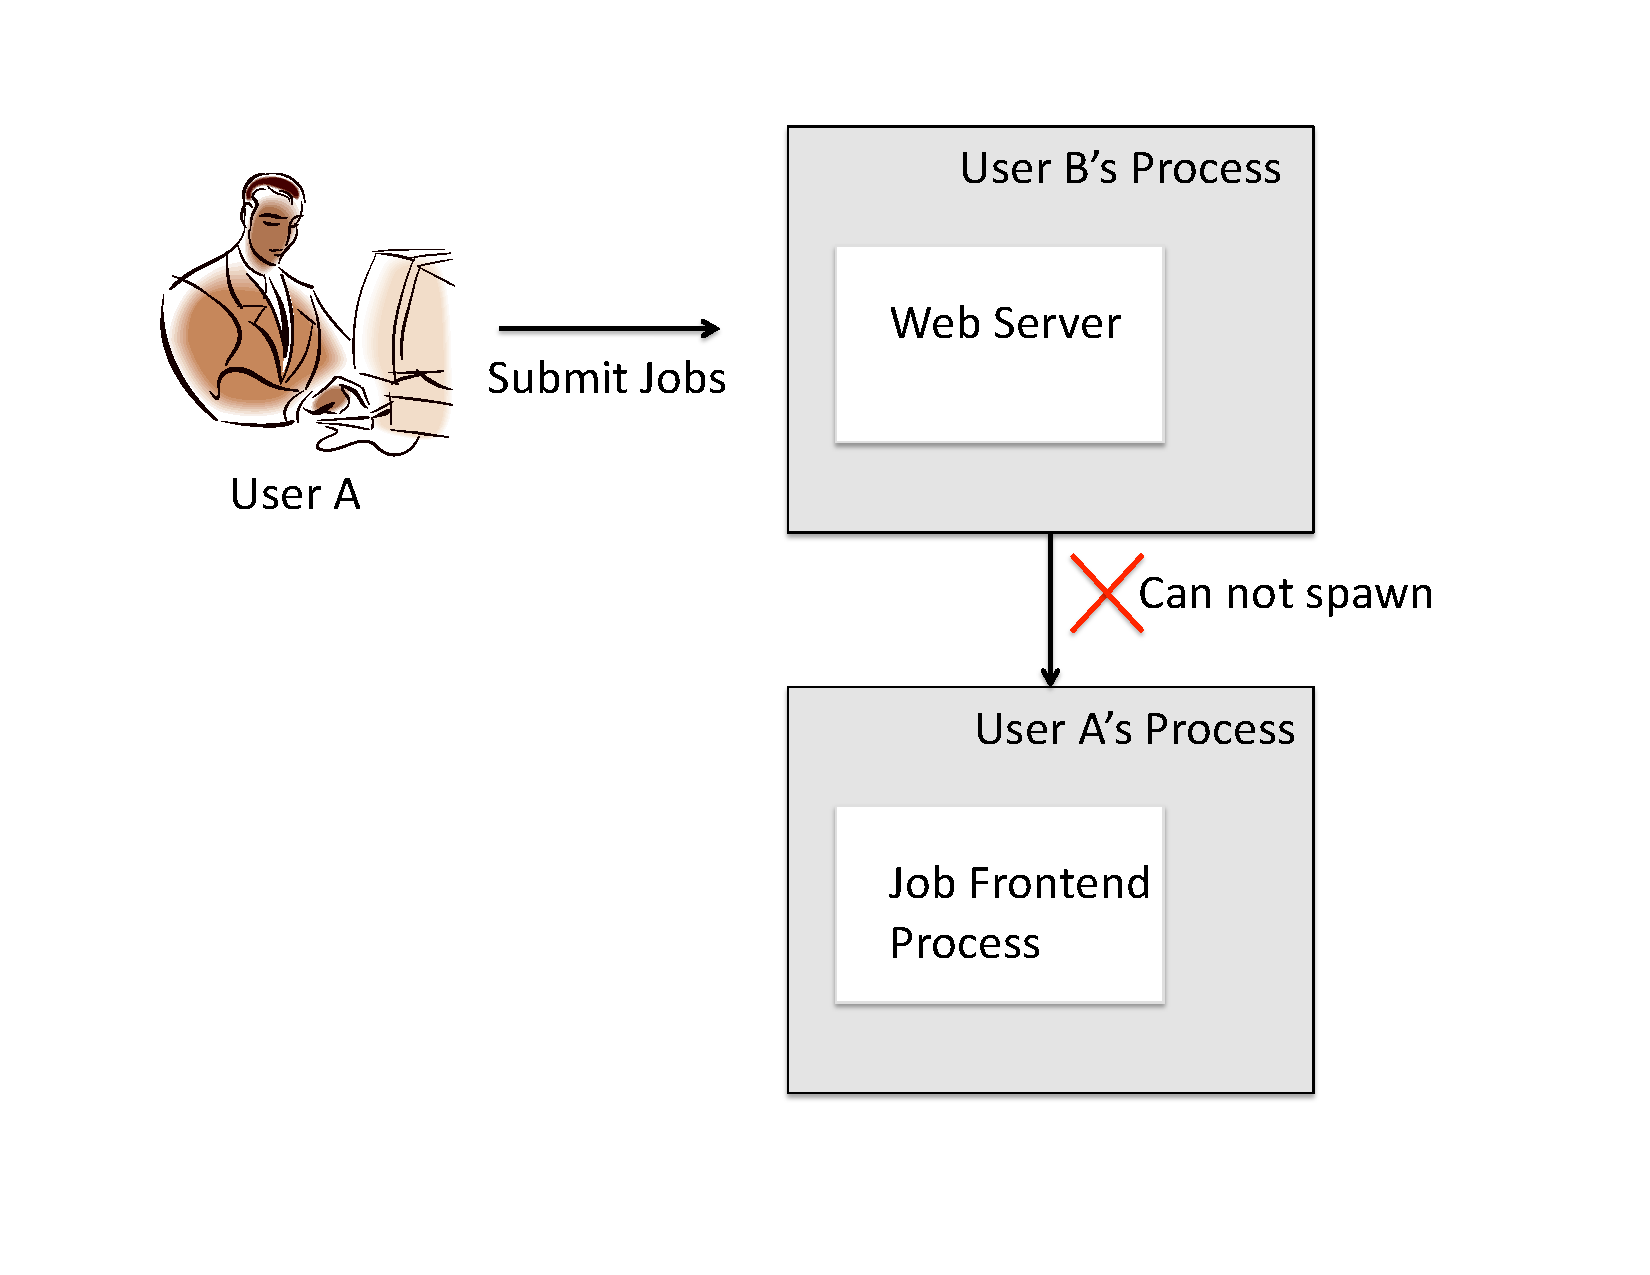
\includegraphics{images/auth_fail}}}}
    %\subfigure[b]{\label{F:dvfs2}{\resizebox{0.3\linewidth}{!}{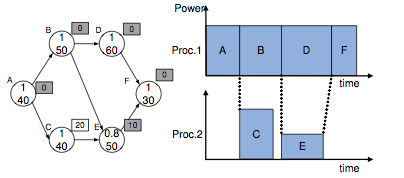
\includegraphics{images/dvfs2}}}}
    \subfigure[Spawn the user's process sucessfully]{\label{F:auth_succ}{\resizebox{0.55\linewidth}{!}{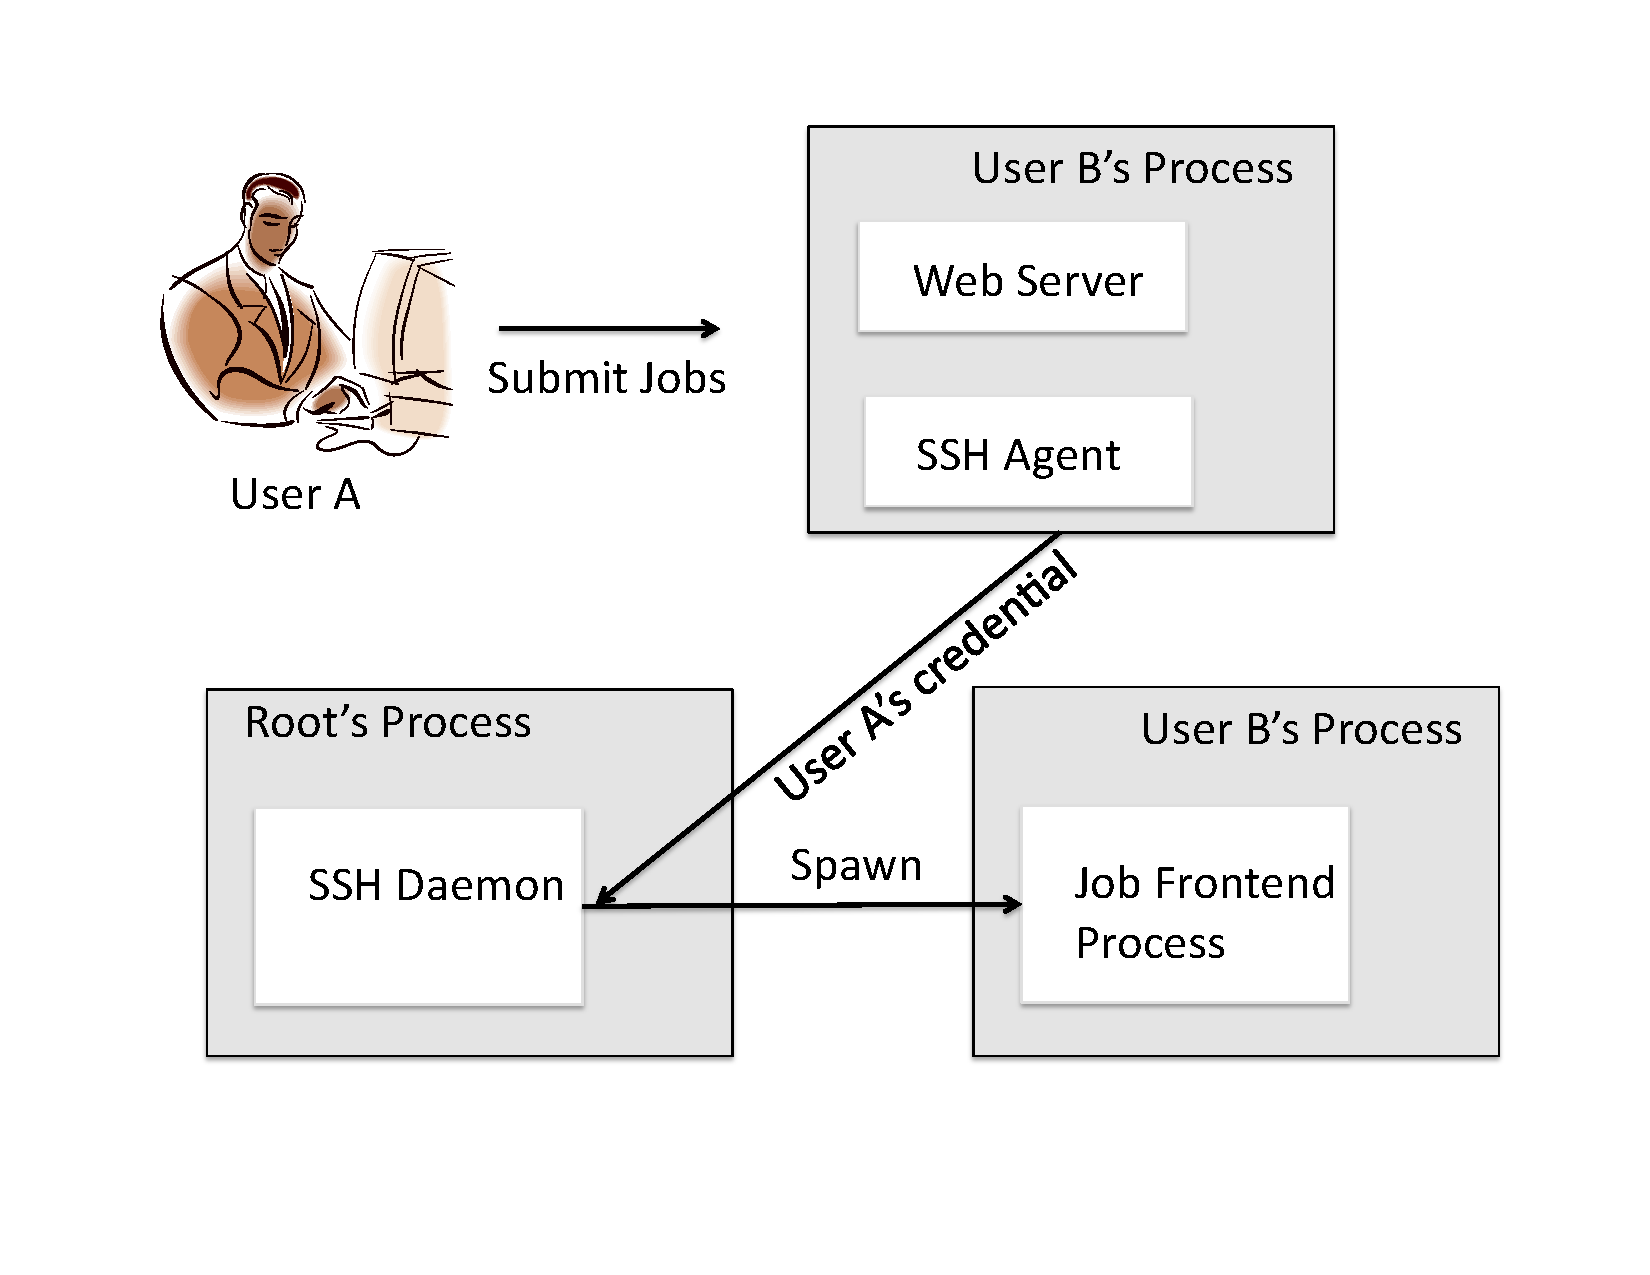
\includegraphics{images/auth_succ}}}}
    }
\caption {A scenario illustrating how to spawn Web interface users' process }
\label {F:auth}
\end{figure}
One of our motivations for redesigning the Web interface is the authentication issues. An important design principles in PJ is that no root privilege is required to start PJ. However, this principle brings a problem into this Web interface design. Illustrated in Figure \ref{F:auth_fail}, a standard user B starts PJ, and another standard user A submits a job through a Web interface and the job is supposed to run on user A's account. The problem is that  the Web server process belongs to user B and since user B is not the root user, he has no privilege to directly spawn a user A's process. 

Figure \ref{F:auth_succ} shows our solution. The Web server process can SSH to the user A's account on the local machine using user A's username and password, and thus start the SSH daemon, and since the SSH daemon is running on behalf of root users, it can spawn the process running on A's account.


    \FIGURE{!htb}
  {images/sshagent}
  {0.8}
  {SSH Agent}
  {F:sshagent} 
  
To solve the authentication issues, we need to implement a SSH agent that acts like a media between SSH daemon and Web server (Figure \ref{F:sshagent}). It can use the username and password provided by the Web interface users to connect to the SSH daemon. Once successfully connected to SSH daemon, SSH agent can submit commands to SSH daemon and ask SSH daemon to execute these commands on behave of the Web interface users, and finally return the result to those users.  

 \subsubsection{Web Server Design}
There are three things we take more consideration when designing the Web interface for PJ. One is the authentication issues discussed above. Another is performance. Since the Web interface is simply used for displaying information of jobs and computer nodes or performing operations such as job submission,  we think it unnecessary to employ the specific Web servers such as Apache HTTP Server as the Web server for this project. They are too heavy-weight and much resource consuming. Instead, we think a light-weight Web server is more suitable. Lastly, we also think security issue is important because more functionality will be added to the new Web interface, and a more secure Web connection is required to protect critical information from eavesdroppers.

\FIGURE{!htb}
{images/web_server}
{0.7}
{Web server component}
{F:web_server} 

The mini Web server for this project is running as a thread inside the Job Scheduler Daemon. As shown in Figure \ref{F:web_server}, the Web server consists of five components: HttpServer, HttpRequest, HttpResponse, SessionManager and SSH Agent. 

HttpServer component is the most important component in the Web server. It adopts SSL Socket technique to provide a secure connection between the browser and the Web server, thus protecting critical information such as username and password from eavesdroppers. HttpServer component alway listens to HTTP requests. When receiving HTTP requests, it will forward these requests to HTTPRequest component for parsing. Once getting parsed request objects back from HttpRequest component, the HttpServer component tries to service these HTTP requests by functioning in accordance with requested URL.

SessionManager component provides session service for the Web server. The session service regards the HTTP requests with the same cookie ID as from the same user and provides the same context to these HTTP requests. If the HTTP requests are for Web interface users to log into the Web server, SessionManager component generates a new cookie ID and save the pair of this cookie ID and user information object in its cache. SessionManager component  also sends back the new cookie ID to the client. Otherwise SessionManager component checks the cookie values of each upcoming HTTP requests, and compare these cookie IDs with its cached cookie IDs. If the same cookie ID is found in SessionManager component's cache, SessionManager component retrieves the corresponding user information and the HTTP request can be serviced in the context of the user's session.

HttpRequest component is responsible for parsing the incoming messages. It retrieves HTTP headers including cookie ID, and request parameters from the HTTP message, and encapsulates them as a request object for HttpServer component's further handling. Its features include Http 1.0/1.1 support, Cookie support and File Upload support; HttpResponse component is used for encapsulating the response objects and parsing these objects to the outgoing messages; 

SSH Agent component implements SSH protocol's client side and is responsible for interacting with SSH daemon. It connects to SSH daemon over TCP/IP network, authenticates to SSH daemon with the username and password passed from the Web interface user and asks SSH daemon to execute commands on behalf of the Web interface user.   

The following steps show how each part of the Web server works together to enable job submission via Web interface. 
\begin{itemize}
\item When a user tries to access PJ's Web interface, the HttpServer component sets up a SSL connection between the Web server and the browse so that all information transported over this connection is under protection.
\item The user logs in to the Web interface using his username and password. The HttpServer component retrieves the username and password, and passes this user credential to SSH Agent component to authenticates to SSH daemon . Once the user can successfully authenticated to SSH daemon, SessionManager component will generate a cookie ID for the user and also save this cookie ID and the user information into its cache. When this user requests the job submission pages, the SessionManager component can recognize this user and this user does not need to input his username and password again. 
\item The user submits his job via Web interface. HttpServer component receives this HTTP request and forwards this request to HttpRequest component.
\item HttpRequest component parses this HTTP message and retrieves cookie ID, uploaded user programs and job information such as the required number of processors, program name, program argument and the location to save the uploaded programs. HttpRequest component encapsulates this information into a request object and sends this object back to the HttpServer component.
\item HttpServer component forwards the job information to SSH Agent component. After connecting to the SSH daemon, the SSH Agent component can submits the job to the SSH daemon and retrieves the results back to HttpServer component.
\item HttpServer component forwards the results to the HttpResponse component which will be responsible for sending the results to the browser.
\end{itemize}
%SSH agent

%%%%%%%%%%%%%%%%%%%%%%%%%%%%%%%%%%%%%%%%%%%%%%%%%%%%%%%%%%%%%%%%%%%%%%
\section{Implementation Examples\label {S:implementation}}
%%%%%%%%%%%%%%%%%%%%%%%%%%%%%%%%%%%%%%%%%%%%%%%%%%%%%%%%%%%%%%%%%%%%%%

%\subsection{Message Passing framework}
%PJ includes a number of processes running on different computer nodes, and is essentially a distributed system. PJ has a message passing framework to make distributed objects work together. 
%/
%\subsection{MAC random number generator}

%\subsection{File Upload}

%\subsection{SSL Session management}
\subsection{Web Server}
A Web server involves many components, including request parsing component, security component or session component.
 \scriptsize
\begin{verbatim} 
// Secure Socket Layer
private SSLServerSocket getSocket(InetSocketAddress address) throws Exception {
         KeyStore ks = KeyStore.getInstance("JKS");
         ks.load(new FileInputStream(keystore), ksPass);
         KeyManagerFactory kmf = KeyManagerFactory.getInstance("SunX509");
         kmf.init(ks, keyPass);
         SSLContext sslcontext = SSLContext.getInstance("SSLv3");
         sslcontext.init(kmf.getKeyManagers(), null, null);
         ServerSocketFactory ssf = sslcontext.getServerSocketFactory();
         SSLServerSocket serversocket = (SSLServerSocket) ssf.createServerSocket(address.getPort());
         return serversocket;
}
\end{verbatim} 
\normalsize
The {\em getSocket()} function takes the advantage of Java library {\em javax.net.ssl} to create a {\em SSLServerSocket} object and provides the secure connection functionality for the Web server. This function assumes a certificate is already in the same file directory as Web server.

\scriptsize
\begin{verbatim}
Content-Type: multipart/form-data; boundary=---------------------------99266353420430460421358796011
-----------------------------99266353420430460421358796011
Content-Disposition: form-data; name="file"; filename="Aes.jar"
Content-Type: application/java-archive
��..
��..
��..
��..
-----------------------------99266353420430460421358796011--
\end{verbatim} 
\normalsize
The above is the stream format when a file is uploaded from the browser.
\scriptsize
\begin{verbatim}
// Here we upload the actual file contents
byte[] preBytes=readBytes(in);
String prevLine = new String(preBytes);
byte temp1[]=prevLine.getBytes();
byte[] currentBytes=readBytes(in);
String currentLine = new String(currentBytes);
int maxSize = 5000;
byte[] buffer = new byte[maxSize];
int currentSize = 0;
while (true) {
    if (currentLine.contains("--" + boundary + "--")) {
            fout.write(buffer, 0, (currentSize - 1));
            break;
    } else {
            byte[] temp = preBytes;
            if ((temp.length + currentSize) >= maxSize) {
                   fout.write(buffer, 0, currentSize);
                   System.arraycopy(temp, 0, buffer, 0, temp.length);
                   currentSize = temp.length;
             } else {
                   System.arraycopy(temp, 0, buffer, currentSize,temp.length);
                   currentSize = currentSize + temp.length;
             }
     }
     prevLine = currentLine;
     preBytes=currentBytes;
     currentBytes=readBytes(in);
     currentLine = new String(currentBytes);
} 
\end{verbatim} 
\normalsize
The above code parses the stream format and saves the stream to a file.

\subsection{SSH Agent} 
The implementation of SSH agent is very complex and we do not need to reinvent the wheels since there already exist a lot of open source Java implementations of SSH agent. For example, JSch \cite{jsch} is a pure java implementation of SSH2, allowing users integrate its functionality to their programs. We tailed JSch and integrate it to our project. 

  \FIGURE{!htb}
  {images/jsch}
  {0.8}
  {JSch's architecture}
  {F:jsch} 

Figure \ref{F:jsch} shows JSch's architecture. The {\em Jsch} component is responsible for the initialization of JSch and the management of {\em Session} components. The Transport Layer Protocol and User Authentication Layer Protocol are implemented in the {\em Session} component. This component supports different authentication methods. The {\em Channel} component represents various kind of SSH channels over which the users can exchange information with remote machines and execute commands on these remote machines. 
The following codes are from the class {\em SSHAutoLogin}, which is developed to communicate with JSch.
\scriptsize
\begin{verbatim} 
// Constructor
public SSHAutoLogin(String host, String username, String password) throws Exception {
         this.username = username;
         this.password = password;
         this.host = host;
         jsch = new JSch();
         jsch.setKnownHosts(System.getProperty("user.home")+ "/.ssh/known_hosts");
         session = jsch.getSession(this.username, this.host, 22);
}
\end{verbatim} 
\normalsize
Class {\em SSHAutoLogin}'s constructor instantiates a {\em JSch} object and {\em Session} object. 
\scriptsize
\begin{verbatim} 	
// Connect to SSH daemon
public boolean connect() {
         try {
              UserInfo ui = new MyUserInfo();
              ui.setPassword(this.password);
              session.setUserInfo(ui);
              session.connect();
         } catch (Exception e) {
              return false;
         }
         return session.isConnected();
}
\end{verbatim} 
\normalsize	
The {\em connect()} function tries to connect to the SSH Daemon using the provided username and password. SSH protocol provides public key authentication, password authentication, host-based authentication and keyboard authentication. But many OpenSSH servers are configured to support only public key authentication and keyboard authentication. In our project, we modifies JSch's source code to use keyboard authentication while reading the username and password from the browser.
\scriptsize
\begin{verbatim} 
// Execute a command
public void executeCmd(String command) throws Exception {
          if (!session.isConnected()) {
                connect();
           }
          Channel channel = session.openChannel("exec");
          ((ChannelExec) channel).setCommand(command);
          channel.setInputStream(null);
          ((ChannelExec) channel).setErrStream(System.err);
          InputStream in = channel.getInputStream();
          channel.connect();

          byte[] tmp = new byte[1024];
          while (true) {
             while (in.available() > 0) {
                   int i = in.read(tmp, 0, 1024);
                   if (i < 0)
                         break;
                   System.out.print(new String(tmp, 0, i));
              }
              if (channel.isClosed()) {
                   break;
              }
              try {
                   Thread.sleep(1000);
              } catch (Exception ee) {
              }
          }
          channel.disconnect();
}
\end{verbatim} 
\normalsize
The {\em executeCmd()} function creates a channel between local machine and remote machine. Over this channel, it can run a command on remote machine and reads the result back. 
\scriptsize
\begin{verbatim}
// Secure copy from local machine to remote machine
public void scp(String source_file, String dist_file) {
         if (!session.isConnected()) {
              connect();
         }
         FileInputStream fis = null;
         try {
              String command = "scp -p -t " + dist_file;
              Channel channel = session.openChannel("exec");
              ((ChannelExec) channel).setCommand(command);

              OutputStream out = channel.getOutputStream();
              InputStream in = channel.getInputStream();

              channel.connect();

              if (checkAck(in) != 0) {
                    System.exit(0);
              }

              // send "C0644 filesize filename", where filename should not include
              // '/'
              long filesize = (new File(source_file)).length();
              command = "C0644 " + filesize + " ";
              if (source_file.lastIndexOf('/') > 0) {
                    command += source_file.substring(source_file.lastIndexOf('/') + 1);
              } else {
                    command += source_file;
              }
              command += "\n";
              out.write(command.getBytes());
              out.flush();
              if (checkAck(in) != 0) {
                    System.exit(0);
              }

              fis = new FileInputStream(source_file);
              byte[] buf = new byte[1024];
              while (true) {
                   int len = fis.read(buf, 0, buf.length);
                   if (len <= 0)
                        break;
                   out.write(buf, 0, len); // out.flush();
              }
              fis.close();
              fis = null;
              // send '\0'
              buf[0] = 0;
              out.write(buf, 0, 1);
              out.flush();
              if (checkAck(in) != 0) {
                   System.exit(0);
              }
              out.close();
              channel.disconnect();
         } catch (Exception e) {
              System.out.println(e);
              try {
                    if (fis != null)
                    fis.close();
              } catch (Exception ee) {
              }
         }
} 
\end{verbatim} 
\normalsize
The {\em scp} function implements the ``scp'' command which copy a file in the local machine to the remote machine in a secure way. 

\subsection{A List of Files Added or Modified} 
~\\
Newly created files
\begin{itemize}
\item /edu/rit/pj/cluster/JobBackendDaemon.java
\item /edu/rit/pj/cluster/JobBackendDaemonMessage.java
\item /edu/rit/pj/cluster/JobBackendDaemonProxy.java
\item /edu/rit/pj/cluster/JobBackendDaemonRef.java
\item /com/jcraft/jsch/SSHAutoLogin.java
\item /edu/rit/http/SessionManager.java
\end{itemize}

Updated files
\begin{itemize}
\item /edu/rit/pj/cluster/Constants.java
\item /edu/rit/pj/cluster/Message.java
\item /edu/rit/pj/cluster/JobFrontend.java
\item /edu/rit/pj/cluster/JobFrontendRef.java
\item /edu/rit/pj/cluster/JobFrontendMessage.java
\item /edu/rit/pj/cluster/JobFrontendProxy.java
\item /edu/rit/pj/cluster/NonPjJobFrontend.java
\item /edu/rit/pj/cluster/JobScheduler.java
\item /edu/rit/pj/cluster/JobSchedulerMessage.java
\item /edu/rit/pj/cluster/JobSchedulerRef.java
\item /edu/rit/pj/cluster/JobSchedulerProxy.java
\item /edu/rit/pj/cluster/ProcessInfo.java
\item /edu/rit/pj/cluster/test/JobFrontendStub.java 
\item /com/jcraft/jsch/UserAuthKeyboardInteractive.java
\item /edu/rit/http/HttpRequest.java
\item /edu/rit/http/HttpResponse.java
\item /edu/rit/http/HttpServer.java
\item /edu/rit/http/SessionManager.java
\end{itemize}

%%%%%%%%%%%%%%%%%%%%%%%%%%%%%%%%%%%%%%%%%%%%%%%%%%%%%%%%%%%%%%%%%%%%%%
\section{Deploy \label {S:deploy}}
%%%%%%%%%%%%%%%%%%%%%%%%%%%%%%%%%%%%%%%%%%%%%%%%%%%%%%%%%%%%%%%%%%%%%%
We design, develop and debug the PJ project on a Macbook Pro. We now demonstrate how to deploy the PJ project onto real cluster parallel computers. 

The PJ project is under /Users/Xi/Documents/workspace/Parallel\_Java. As shown in Figure \ref{F:folder}, the source codes are organized under {\em src} directory while the binary codes are organized under {\em bin} directory. {\em scheduler.conf} is the configure file and {\em scheduler.log} is the log file.
      
\FIGURE{!htb}
{images/folder.png}
{0.9}
{PJ project directory}
{F:folder}
 
The cluster parallel computer we are going to have PJ run on is located at Computer Science Department, Rochester Institute of Technology. It has one frontend node named {\em paranoia} and thirty two backend nodes named {\em thug01} through {\em thug32}. 
   
\subsection*{Packaging and Copying}
\begin{enumerate}
\item Open a terminal window, and go to the binary code directory.
\begin{verbatim} 
$ cd /Users/Xi/Documents/workspace/Parallel_Java/bin
\end{verbatim}
\item Package the class files into a jar file.
\begin{verbatim} 
$ jar -cvf pj.jar *
\end{verbatim}
\item Copy the jar file to {\em paranoia}
\begin{verbatim} 
$ scp pj.jar xxh2229@paranoia.cs.rit.edu:/var/tmp/parajava_test
\end{verbatim}
SSH to paranoia, and copy {\em pj.jar} to 32 backend nodes using the similar command.
\begin{verbatim} 
$ ssh xxh2229@paranoia.cs.rit.edu
$ cd /var/tmp/parajava_test
$ scp pj.jar xxh2229@thug01:/var/tmp/parajava_test
$ ......
$ ......
$ scp pj.jar xxh2229@thug32:/var/tmp/parajava_test
$ exit
\end{verbatim}
\item Copy the configure and log file to {\em paranoia}
\begin{verbatim} 
$ scp scheduler.conf xxh2229@paranoia.cs.rit:/var/tmp/parajava_test
$ scp scheduler.log xxh2229@paranoia.cs.rit:/var/tmp/parajava_test
\end{verbatim}
\end{enumerate}

\subsection*{Configuration File}
The following lists the content of {\em scheduler.conf}. This file records the configuration for both the frontend node and the backend nodes. For example, it specifies the location of the log file, the hostname and the port of both the Web interface and the Job Scheduler Daemon as well as the hostname of the Job Frontend Process. The original version of PJ specifies the hostname of the Job Scheduler Daemon as ``localhost'' because in that version the Job Scheduler Daemon only communicates with the Job Frontend Process which is running on the same node as the Job Scheduler Daemon. However, in the new version of PJ, the Job Scheduler Daemon not only communicate with the Job Frontend Process but also with the Job Backend Daemon running on different computer nodes, we need to specify a full domain name for the Job Scheduler Daemon.

The {\em scheduler.conf} also specifies each backend node'  machine name and full domain name as well as the location of Java virtual machine and PJ library in these backend nodes.
%\begin{lstlisting}[caption=scheduler.conf,
%  label=scheduler,
%  float=t]
\scriptsize
\begin{verbatim} 
# Parallel Java Job Scheduler configuration file
# Frontend processor: paranoia
# Backend processors: thug01-thug32

cluster RIT CS Paranoia 32-Processor Cluster
logfile /var/tmp/parajava_test/scheduler.log
webhost paranoia.cs.rit.edu
webport 8082
schedulerhost paranoia.cs.rit.edu
schedulerport 20618
frontendhost paranoia.cs.rit.edu
backend thug01 1 thug01 /usr/jdk/jdk1.5.0_23/bin/java /var/tmp/parajava_test/pj.jar -server
backend thug02 1 thug02 /usr/jdk/jdk1.5.0_23/bin/java /var/tmp/parajava_test/pj.jar -server
backend thug03 1 thug03 /usr/jdk/jdk1.5.0_23/bin/java /var/tmp/parajava_test/pj.jar -server
backend thug04 1 thug04 /usr/jdk/jdk1.5.0_23/bin/java /var/tmp/parajava_test/pj.jar -server
backend thug05 1 thug05 /usr/jdk/jdk1.5.0_23/bin/java /var/tmp/parajava_test/pj.jar -server
backend thug06 1 thug06 /usr/jdk/jdk1.5.0_23/bin/java /var/tmp/parajava_test/pj.jar -server
backend thug07 1 thug07 /usr/jdk/jdk1.5.0_23/bin/java /var/tmp/parajava_test/pj.jar -server
backend thug08 1 thug08 /usr/jdk/jdk1.5.0_23/bin/java /var/tmp/parajava_test/pj.jar -server
backend thug09 1 thug09 /usr/jdk/jdk1.5.0_23/bin/java /var/tmp/parajava_test/pj.jar -server
backend thug10 1 thug10 /usr/jdk/jdk1.5.0_23/bin/java /var/tmp/parajava_test/pj.jar -server
backend thug11 1 thug11 /usr/jdk/jdk1.5.0_23/bin/java /var/tmp/parajava_test/pj.jar -server
backend thug12 1 thug12 /usr/jdk/jdk1.5.0_23/bin/java /var/tmp/parajava_test/pj.jar -server
backend thug13 1 thug13 /usr/jdk/jdk1.5.0_23/bin/java /var/tmp/parajava_test/pj.jar -server
backend thug14 1 thug14 /usr/jdk/jdk1.5.0_23/bin/java /var/tmp/parajava_test/pj.jar -server
backend thug15 1 thug15 /usr/jdk/jdk1.5.0_23/bin/java /var/tmp/parajava_test/pj.jar -server
backend thug16 1 thug16 /usr/jdk/jdk1.5.0_23/bin/java /var/tmp/parajava_test/pj.jar -server
backend thug17 1 thug17 /usr/jdk/jdk1.5.0_23/bin/java /var/tmp/parajava_test/pj.jar -server
backend thug18 1 thug18 /usr/jdk/jdk1.5.0_23/bin/java /var/tmp/parajava_test/pj.jar -server
backend thug19 1 thug19 /usr/jdk/jdk1.5.0_23/bin/java /var/tmp/parajava_test/pj.jar -server
backend thug20 1 thug20 /usr/jdk/jdk1.5.0_23/bin/java /var/tmp/parajava_test/pj.jar -server
backend thug21 1 thug21 /usr/jdk/jdk1.5.0_23/bin/java /var/tmp/parajava_test/pj.jar -server
backend thug22 1 thug22 /usr/jdk/jdk1.5.0_23/bin/java /var/tmp/parajava_test/pj.jar -server
backend thug23 1 thug23 /usr/jdk/jdk1.5.0_23/bin/java /var/tmp/parajava_test/pj.jar -server
backend thug24 1 thug24 /usr/jdk/jdk1.5.0_23/bin/java /var/tmp/parajava_test/pj.jar -server
backend thug25 1 thug25 /usr/jdk/jdk1.5.0_23/bin/java /var/tmp/parajava_test/pj.jar -server
backend thug26 1 thug26 /usr/jdk/jdk1.5.0_23/bin/java /var/tmp/parajava_test/pj.jar -server
backend thug27 1 thug27 /usr/jdk/jdk1.5.0_23/bin/java /var/tmp/parajava_test/pj.jar -server
backend thug28 1 thug28 /usr/jdk/jdk1.5.0_23/bin/java /var/tmp/parajava_test/pj.jar -server
backend thug29 1 thug29 /usr/jdk/jdk1.5.0_23/bin/java /var/tmp/parajava_test/pj.jar -server
backend thug30 1 thug30 /usr/jdk/jdk1.5.0_23/bin/java /var/tmp/parajava_test/pj.jar -server
backend thug31 1 thug31 /usr/jdk/jdk1.5.0_23/bin/java /var/tmp/parajava_test/pj.jar -server
backend thug32 1 thug32 /usr/jdk/jdk1.5.0_23/bin/java /var/tmp/parajava_test/pj.jar -server
jobtime 3600
\end{verbatim} 
\normalsize
%\end{lstlisting}

\subsection*{Setting Up A Certificate For The Web Server }
\begin{enumerate}
\item Generate a certificate
\begin{verbatim} 
$ keytool -genkey -keystore paralleljava.ks \
>  -keyalg rsa -alias parallel
\end{verbatim}
\item Copy the certificate to {\em paranoia}
\begin{verbatim} 
$ scp paralleljava.ks xxh2229@paranoia.cs.rit:/var/tmp/parajava_test
\end{verbatim}
\item SSH to paranoia, and make this certificate only readable and writable by its owner
\begin{verbatim} 
$ ssh xxh2229@paranoia.cs.rit.edu
$ cd /var/tmp/parajava_test
$ chmod 600 paralleljava.ks
\end{verbatim}
\end{enumerate}

%%%%%%%%%%%%%%%%%%%%%%%%%%%%%%%%%%%%%%%%%%%%%%%%%%%%%%%%%%%%%%%%%%%%%%
\section{User Manual \label {S:usermanual}}
%%%%%%%%%%%%%%%%%%%%%%%%%%%%%%%%%%%%%%%%%%%%%%%%%%%%%%%%%%%%%%%%%%%%%%
This user manual is for each PJ user to configure their accounts before they can correctly use the cluster parallel computers.
\subsection*{Setting Up Users' Account}
\begin{enumerate}
\item Create .ssh directory
\begin{verbatim} 
$ mkdir .ssh
\end{verbatim}
\item Copy the known\_files file to .ssh directory
\begin{verbatim} 
$ cd .ssh
$ cp /home/fac/ark/public_html/known_hosts .
\end{verbatim}
\item Generate RSA keys.
\begin{verbatim} 
$ ssh-keygen -t rsa
$ cp id_rsa.pub authorized_keys
\end{verbatim}
\item Generate authentication keys. Randomly generate 32 characters and save these characters into a file name ``key'' under .ssh/hmac/
\item Make .ssh directory and the files in it only readable and writable to their owner
\begin{verbatim} 
$ chmod 600 *
$ chmod 700 .
\end{verbatim}
\end{enumerate}

\subsection*{Submit the jobs from command line}
Suppose that we are going to submit a java file named {\em AesTestClu.java} to {\em paranoia}.
\begin{enumerate}
\item Upload the java file
\begin{verbatim} 
$ scp Aesclu.java xxh2229@paranoia.cs.rit:~
\end{verbatim}
\item Set up the classpath
\begin{verbatim} 
$ export CLASSPATH=.:/var/tmp/parajava_test/pj.jar
\end{verbatim}
\item Compile the java file
\begin{verbatim} 
$ /usr/local/versions/jdk-1.5.0_15/bin/javac AesClu.java
\end{verbatim}
\item Run the program on 8 processors.
\begin{verbatim} 
$ KEY=55e1360d5115bc403d03e32571163f29a0f86f41817e8290d4c13e8d8f311fe3
$ /usr/jdk/jdk1.5.0_17/bin/java -Dpj.np=8 AesTestClu $KEY 750000
\end{verbatim}
\item Get the result. (Figure \ref{F:commandline1})
\FIGURE{!htb}
{images/commandline1.png}
{0.8}
{The result after running the submitted program}
{F:commandline1}
\end{enumerate}

\subsection*{Submit the jobs from the Web interface}
\begin{enumerate}
\item Go to the PJ Web interface. (Type ``https://paranoia.cs.rit.edu:8082/'' in the browser's address bar)
%\FIGURE{!htb}
%{images/webportal1.png}
%{1}
%{Web site for PJ Web interface}
%{F:webportal1}
\item A warning window pops up (Figure \ref{F:webportal2}). That is because currently our certificate is not certified by any certificate authority. Select ``Continue''.
\FIGURE{H}
{images/webportal2.png}
{0.8}
{A warning window}
{F:webportal2}
\item PJ's Web interface show the status of the cluster parallel computers and the jobs. (Figure \ref{F:webportal3})
\FIGURE{H}
{images/webportal3.png}
{0.8}
{PJ Web interface's main page}
{F:webportal3}
\item Login to PJ Web interface using the same credential as logging in to {\em paranoia}. (Figure \ref{F:webportal4}, \ref{F:webportal5})
\FIGURE{H}
{images/webportal4.png}
{0.8}
{Login window}
{F:webportal4}

\FIGURE{H}
{images/webportal5.png}
{0.8}
{My PJ Web interface}
{F:webportal5}
\item Provide the necessary job information, and submit the job to {\em paranoia} .(Figure \ref{F:webportal6})
\FIGURE{H}
{images/webportal6.png}
{0.8}
{logged page}
{F:webportal6}
\item Get the result back.(Figure \ref{F:webportal7})
\FIGURE{H}
{images/webportal7.png}
{0.8}
{logged page}
{F:webportal7}
\end{enumerate}

%%%%%%%%%%%%%%%%%%%%%%%%%%%%%%%%%%%%%%%%%%%%%%%%%%%%%%%%%%%%%%%%%%%%%%
\section{Test Runs\label {S:test}}
%%%%%%%%%%%%%%%%%%%%%%%%%%%%%%%%%%%%%%%%%%%%%%%%%%%%%%%%%%%%%%%%%%%%%%
%To test the performance of different job launching schemes, we measure the time for these job launching schemes take to start executing jobs. The test program is the programming project in the course of Parallel Computing I. The program conducts a statistical test to try to disprove that Advanced Encryption Standard(AES) behaves as a random function. Two input parameters are required. One is a 64-hexadecimal-digit number key for AES encryptions. The other one is the number of plaintext blocks N. The command for compiling and running the program is as follows:

%\begin{verbatim} 
%$ export CLASSPATH=.:/var/tmp/parajava_test/pj.jar
%$ /usr/local/versions/jdk-1.5.0_15/bin/javac AesClu.java
%$ KEY=55e1360d5115bc403d03e32571163f29a0f86f41817e8290d4c13e8d8f311fe3
%$ /usr/jdk/jdk1.5.0_17/bin/java -Dpj.np=32 AesTestClu $KEY 750000
%\end{verbatim}

To evaluate the new job launching scheme and Web interface's performance, we run the parallel program using four job launching schemes and measure the time for these schemes to start launching the program.  These four job launching schemes include PJ's original job launching scheme, PJ's new job launching scheme, PJ's Web Interface and Sun's MPI job launching scheme. 

The program we use for the test is to implement Floyd's algorithm to calculate the length of the shortest path from each node to every other node in a network. We run this program 10 times on the cluster parallel computers  and record the time to start launching the program. For the job launching schemes related to PJ, we start the measurement when the Job Frontend Process requests resource from the Job Scheduler Daemon, and end the measurement when the Job Backend Processes start executing jobs. For Sun's MPI job launching scheme, we start the measurement when the user submits the program to {\em paranoia} and end the measurement before the backend nodes start to execute the {\em MPI\_Init} command.

\FIGURE{H}
{images/pj}
{0.9}
{Measurement}
{F:pj}

The result (Figure \ref{F:pj}) is excellent. Efficiency of the new job launching scheme and Web interface is almost the same, and that is because they are all based on PJ's new job launching scheme.  From the second job, the time for the new job launching scheme to launch the job decreases drastically, about one tenth of the time used by the original job launching scheme. The reason is that once the Job Backend Daemon starts, the Job Frontend Process can use MAC base message passing to communicate with Job Backend Daemon and spawn the Job Backend Process via Job Backend Daemon. This scheme is much more faster than that based on SSH. 

The result also shows that Sun's MPI job launching scheme is even faster than PJ's new job launching scheme, probably because Sun's MPI job launching scheme is based on C and uses low level and more efficient message passing methods. Another interesting observation is that it takes apparently more time for Sun's MPI to start launching jobs for the first time.
%%%%%%%%%%%%%%%%%%%%%%%%%%%%%%%%%%%%%%%%%%%%%%%%%%%%%%%%%%%%%%%%%%%%%%
\section{Future Work \label {S:futurework}}
%%%%%%%%%%%%%%%%%%%%%%%%%%%%%%%%%%%%%%%%%%%%%%%%%%%%%%%%%%%%%%%%%%%%%%
While the new job launching scheme and Web interface in their current shape is fully functional and useful, there is still room for improvement.

The Web interface is based on SSL, but its certificate is not certified by any certificate authority. As a result, there is a potential danger for Web interface users when they visit the Web interface and accept the Web interface certificate. Because others can pretend to be PJ's Web interface and put the Web interface users at risk. In addition, there are still room for improving the Web interface, for example, adding the functionality that allow users to cancel their jobs or retrieve their output files.
%%%%%%%%%%%%%%%%%%%%%%%%%%%%%%%%%%%%%%%%%%%%%%%%%%%%%%%%%%%%%%%%%%%%%%
\section{Conclusion \label {S:conclusion}}
%%%%%%%%%%%%%%%%%%%%%%%%%%%%%%%%%%%%%%%%%%%%%%%%%%%%%%%%%%%%%%%%%%%%%%
The project is very successful. The new job launching scheme shortens time for PJ to start launching the submitted jobs by 10 times compared to the original one. The improved Web interface provides more services to PJ users and PJ users can easily submit their jobs to PJ.

More significance for this project is that we achieve a lot while working on the project. We are exposed to a bunch of classical computing paradigm such as distributed system, parallel computing. We study SSH protocol, HTTP protocol, and we even design our protocol for communication between various processes. We get a deeper understanding of MAC. We get familiar with Java language and its related library. We also gain much experience in designing and developing a software system.


